\begin{exercice}
    Soit $f$ une fonction dérivable sur $[0, 1]$ telle que:
    $$f(0) = f'(0) = f'(1) = 0 \text{ et } f(1) = 1.$$
    Montrer qu'il existe $c \in ]0, 1[$ tel que $f(c) = c$. 
\end{exercice}

\begin{elem_sol}
    \begin{itemize}
        \item Poser $g(x)= f(x) - x$.
        \item L'objectif est de montrer que $g$ s'annule au moins une fois sur $[0, 1]$ en montrant l'existence de $x_0$ et $x_1$ dans $[0, 1]$ tels que $g(x_0) < 0$ et $g(x_1) > 0$ pour pouvoir appliquer le \textbf{théorème des valeurs intermédiaires}.
        \item Raisonner par l'absurde sur l'existence de $x_0$ et de $x_1$ et écrire la dérivée de $f$ comme la limite de son taux d'accroissement pour aboutir à des contradictions. 
    \end{itemize}
\end{elem_sol}

\begin{marginfigure}[-7cm]
\centering
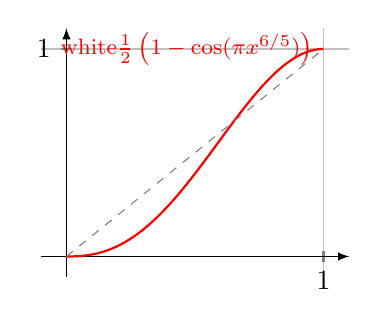
\begin{tikzpicture}
    \begin{axis}[width=5.5cm,
        axis lines=middle,
        axis line style={-latex},
        grid=major,
        xmin=-0.1, xmax=1.1,
        ymin=-0.1, ymax=1.1,
        xtick={0,1},
        xticklabels={$0$, $1$},
        ytick={0,1},
        yticklabels={$0$, $1$},
        tick style={thick},
        ticklabel style={font=\normalsize},
    ]
    \def\a{0}
    \def\b{1}
    \addplot[red,thick,samples=100,domain=\a:\b] {1/2*(1-cos(deg(pi*x^1.2)))}
    node[left,pos=1,font=\footnotesize]{\contour{white}{$\frac{1}{2} \left(1-\cos (\pi x^{6/5}) \right)$}};
    \addplot[gray,dashed,samples=100,domain=\a:\b] {x};
    \end{axis}
\end{tikzpicture}
\caption*{\centering Exemple d'une fonction vérifiant les hypothèses de l'énoncé}
\end{marginfigure}

